\subsection{From competitive provision to monopoly with RSI}
\label{subsec:rewrite-competitive-transition}

I now examine a different experiment: granting exclusive rights over AI
technology in an economy that initially supplies AI services competitively.
This allows me to compare the initial restriction in AI use with the
subsequent efficiency gains financed by monopoly rents. Unlike the
preceding exercises, RSI is available before date zero, with the same
positive $\chi$ as after the change. Research is nevertheless zero under
the free-access arrangement in Section~\ref{sec:rewrite-competition},
because improvements cannot be privately appropriated.

I retain the parameters in Table~\ref{tab:rewrite-rsi-parameters}, including
both research productivities and all four elasticities, but choose $K_0$
to place each economy on its competitive BGP at the same $B_0$. Before
the change, $p_X=1/B_0$, $r=\rho+\gamma$, and $K_0/Y_0=3.3$.
Table~\ref{tab:rewrite-competitive-transition} reports the new capital
stocks. In every case, continued competition would preserve the
labor-bottleneck BGP, with output per worker, consumption per person,
and wages growing at $\gamma$.

At date zero, an unexpected permanent exclusive right covers both the
existing AI technology and its subsequent improvements. In particular,
competitive suppliers can no longer use the old technology. The economy
then follows the monopoly equilibrium, inheriting $K_0$ and $B_0$ but
choosing consumption and research anew. This experiment changes research
incentives and pricing, not the RSI technology. It abstracts from the
cost of enforcing exclusivity and is not an optimal policy exercise.

\begin{table}[H]
 \centering
 \caption{Competitive initial capital and the impact of exclusive AI rights}
 \label{tab:rewrite-competitive-transition}
 \small\setstretch{1.0}
 \begin{tabular}{cccc}
 \toprule
 $\sigma$ & $K_0$ & Change in output & Change in wage\\
 \midrule
 0.9 & 6.235 & $-32.4\%$ & $-36.6\%$\\
 1.0 & 6.278 & $-17.6\%$ & $-17.6\%$\\
 1.1 & 6.324 & $-13.7\%$ & $-11.9\%$\\
 1.5 & 6.535 & $-10.4\%$ & $-5.4\%$\\
 \bottomrule
 \end{tabular}
 \par\vspace{4pt}
 \parbox{0.95\textwidth}{\footnotesize\emph{Notes:} The capital stocks are
 derived from the competitive BGP, not selected independently. All other
 parameters and initial stocks are in Table~\ref{tab:rewrite-rsi-parameters}.
 Changes compare levels immediately after and before the grant. They are
 identical for both values of $\chi$, since $K$ and $B$ cannot jump.
 The ratio $K_0/Y_0=3.3$ applies before the grant, not after output falls.}
\end{table}

I first consider $\chi=7.5$ in
Figure~\ref{fig:rewrite-competitive-high-levels}. Panels A--C show output
per worker, wages, and consumption per person, each relative to continued
competition from the same initial stocks. The line styles identify the
four elasticities as in the preceding figures. The upper row includes
two pre-event years and years 0--10; the middle row shows years 10--100;
the lower row shows years 10--500. The competitive benchmark is
$100.0\%$ in the upper row and one in the logarithmic lower rows.
The intermediate window makes recoveries visible that would be
compressed in the 500-year view.

The initial markup reduces AI use, output, and wages before efficiency
can improve. At $\sigma=1.5$, output and wages fall by $10.4\%$ and
$5.4\%$, respectively. Research subsequently raises efficiency, and
output first regains its competitive counterpart around year 3.8;
wages do so around year 4.6. Consumption instead rises by $8.2\%$ at
the grant, even as output falls. The household chooses less capital
accumulation, while reduced inference use releases some resources.
The consumption response therefore need not have the same sign as the
output response.

\begin{figure}[H]
 \centering
 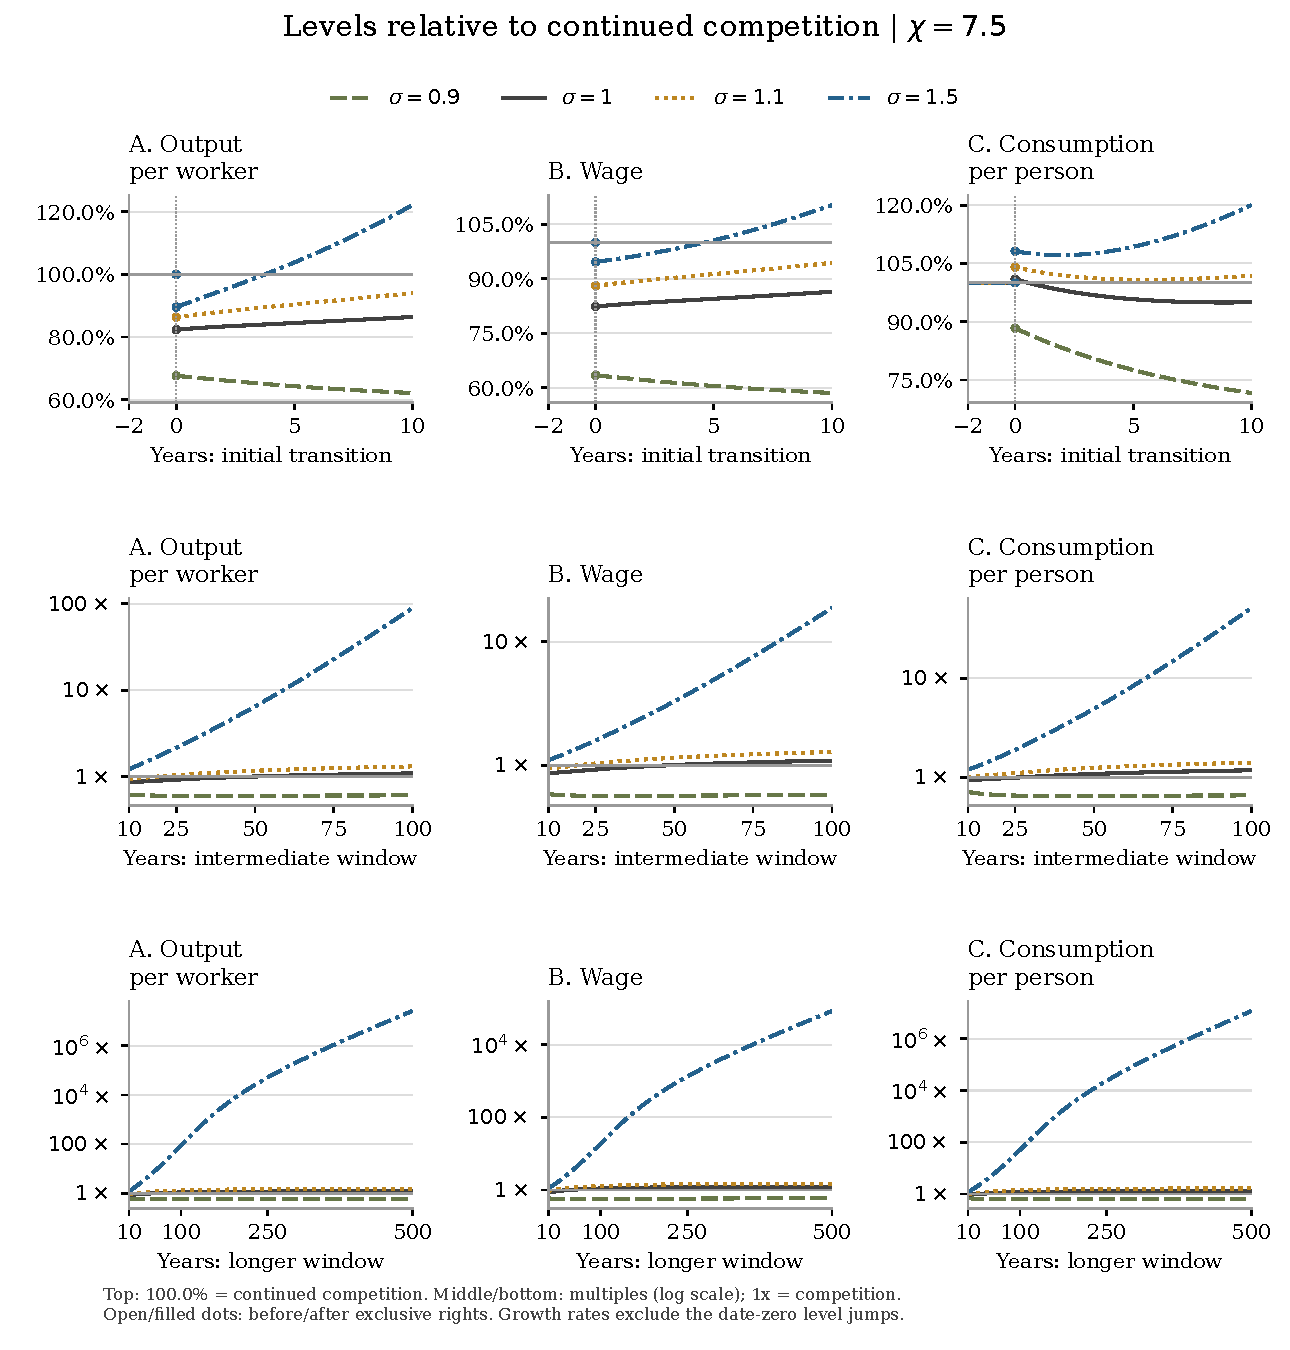
\includegraphics[width=\textwidth]{figures_rewrite/competitive_to_monopoly/competitive_to_monopoly_chi_7_5_levels.pdf}
 \caption{From competition to monopoly with RSI, $\chi=7.5$: levels
 relative to continued competition. The rows cover years $-2$--10,
 10--100, and 10--500. The upper row uses percentages; the middle and
 lower rows use multiples on logarithmic scales. The horizontal
 benchmark is $100.0\%$ or $1\times$. Open and filled dots mark levels
 before and after the grant. Vertical scales differ across windows
 and between the two research-productivity exercises.}
 \label{fig:rewrite-competitive-high-levels}
\end{figure}

The middle row shows that recovery is not confined to the AI-dominated
case. Output catches up around year 18.2 at $\sigma=1.1$ and year 46.9
at $\sigma=1$. These economies obtain level gains even though their
long-run output-per-worker and wage growth return to $\gamma$.
By contrast, the lower row shows an expanding gap at $\sigma=1.5$:
the monopoly economy approaches the AI-dominated regime, while the
competitive counterfactual remains labor-bottlenecked. At $\sigma=0.9$,
neither output nor wages recover within 500 years. Higher AI efficiency
does not necessarily compensate for restricted access to AI services.

I next lower research productivity to $\chi=1.5$ in
Figure~\ref{fig:rewrite-competitive-low-levels}, using the same stocks,
comparison, and time windows. The initial output and wage losses are
unchanged, but research absorbs less output: at $\sigma=1.5$, its initial
share is $0.6\%$ rather than $3.3\%$. Consumption initially rises by
$3.7\%$ rather than $8.2\%$. Lower research productivity thus changes
the initial allocation as well as the speed of subsequent improvement.
Output and wages at $\sigma=1.5$ remain below the competitive benchmark
throughout the first decade, recovering only around years 24.0 and
26.0. Output at $\sigma=1.1$ recovers around year 87.3, whereas at
$\sigma=1$ recovery falls outside the intermediate window, around
year 212.3.

\begin{figure}[H]
 \centering
 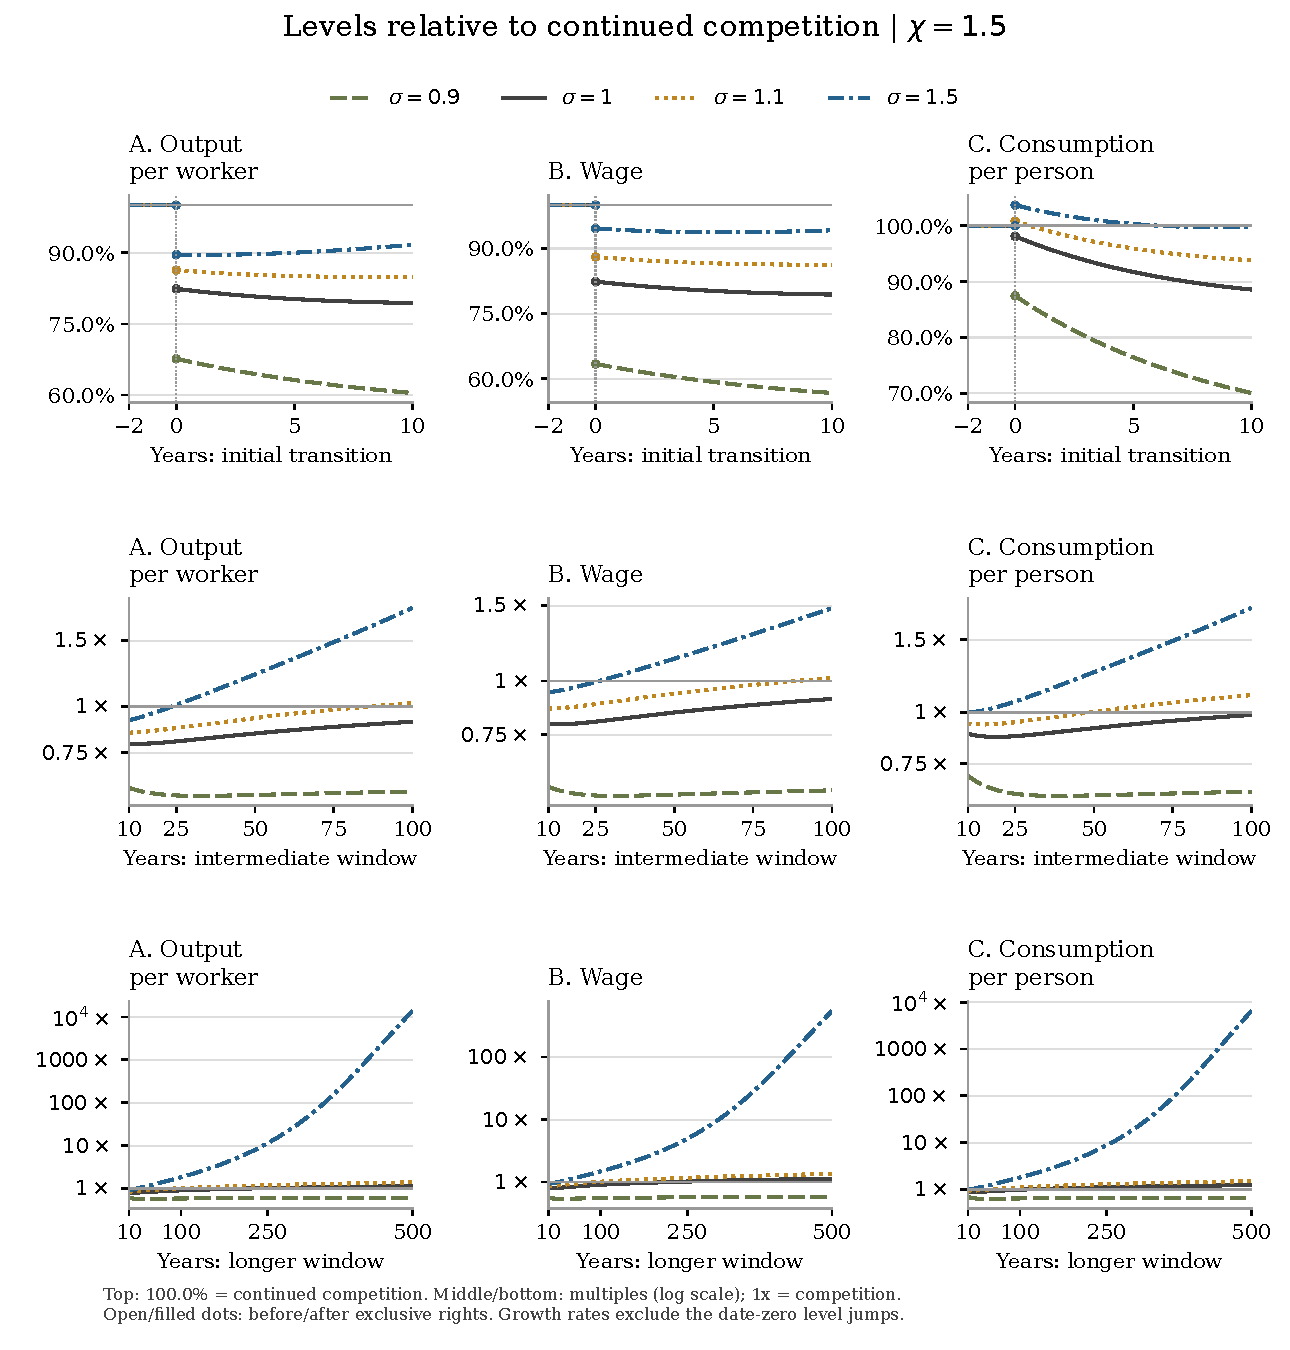
\includegraphics[width=\textwidth]{figures_rewrite/competitive_to_monopoly/competitive_to_monopoly_chi_1_5_levels.pdf}
 \caption{From competition to monopoly with RSI, $\chi=1.5$: output
 per worker, wages, and consumption per person relative to continued
 competition. Windows, normalizations, and line styles match
 Figure~\ref{fig:rewrite-competitive-high-levels}; vertical scales are
 fitted to this exercise. The middle row reveals recoveries outside
 the first decade, while the lower row retains the longer transition.}
 \label{fig:rewrite-competitive-low-levels}
\end{figure}

Research productivity changes these recoveries, not the monopoly limits
in Proposition~\ref{prop:rewrite-equilibrium-regimes}. At $\sigma=1.5$,
limiting output-per-worker growth, wage growth, and the interest rate
are $3.1\%$, $2.4\%$, and $7.1\%$ under either $\chi$. The lower rows
show the separation from continued competition, not completed
convergence: the interest rate at year 500 is still $7.2\%$ with high
research productivity and $8.2\%$ with low research productivity.
Appendix~\ref{app:rewrite-competitive-transition} reports growth,
prices, income shares, and compute expenditure for all eight paths.

I interpret these simulations as an institutional counterfactual, not
as a calibrated prediction of granting AI exclusivity. In particular,
the impact price at $\sigma=0.9$ is about 131 times its competitive
level, a large distortion implied by the inherited parameters.
The recovery dates compare contemporaneous levels, not cumulative
gains or household welfare. Evaluating the policy would require the
entire consumption path, not just the date at which output or wages
overtake continued competition.
